% *** LaTeX-mal for labrapporter i fysikk, v.14.08.2017 ***

% Dette er et eksempel på et LaTeX-dokument, og du kan bruke dette som et utgangspunkt for din egen rapport. Merk at for å kunne kompilere dokumentet uten feil, må du også laste ned filen pendel-oppdatert.pdf.
%
% Her i starten og videre nedover i teksten under har vi lagt inn en god del linjer som starter med tegnet "%". Disse linjene er kommentarer og synes ikke i det ferdige dokumentet. Vi kan også sette inn et kommentartegn midt på en linje. Alt som kommer før tegnet brukes da i kompileringen, mens resten av linja er en kommentar. 
%
% Kildefilen (.tex-filen) begynner alltid med et "preabmle". Her setter man opp innstillingene som brukes av kompilatoren til å utforme det ferdige dokumentet. Selve dokumentet begynner ikke før vi skriver \begin{document}.
%
% Dokumentasjon for alle pakker finnes på CTAN (http://www.ctan.org/)

%%%%%%%%%%%%%%%%%%%%%%%%%%%%%%%%%%%%%
% Preamble
%%%%%%%%%%%%%%%%%%%%%%%%%%%%%%%%%%%%%

\documentclass[5p,sort&compress]{elsarticle}		
% 5p gir 2 kolonner pr side. 1p gir 1 kolonne pr side.
% Valget sort&compress gjør at referansen [1,2,3] settes som [1-3]. 
% Andre innstillinger for "klassen" elsarticle finnes i dokumentasjonen på CTAN (http://www.ctan.org/pkg/elsarticle)

% Klassen elsarticle er laget for bruk i engelskspråklige tiksskrift. I blokken under bruker vi litt lavnivå TeX-magi for å redefinere bunnteksten på tittelsiden. Ikke bekymre deg for denne biten med kode, det som kommer lengere nede i dokumentet er lettere å forstå!
\makeatletter
\def\ps@pprintTitle{%
 \let\@oddhead\@empty
 \let\@evenhead\@empty
 \def\@oddfoot{\footnotesize\itshape
       Utkast levert til Veileder	% Bytt ut "Veileder" med navnet på veilederen din!
       \hfill\today}%
 \let\@evenfoot\@oddfoot}
\makeatother

% Encoding for input i tex-filen og encoding for output i pdf-filen
\usepackage[utf8]{inputenc}
\usepackage[T1]{fontenc}
\usepackage{textcomp}

% Last inn en font-pakke. Her bruker vi standard-fonten til LaTeX. 
\usepackage{lmodern}

% LaTeX gjør mye av typografien for deg, blant annet orddeling ved linjeskift og automatisk utfylling av endel tekst. For å kunne gjøre dette må kompilatoren vite hvilket språk dokumentet er skrevet på. 
\usepackage[norsk]{babel}
\usepackage[fixlanguage]{babelbib}
% Til tross for at vi har fortalt kompilatoren at vi skriver på norsk må vi fortelle den eksplisitt at vi ønsker at seksjonen "abstract" skal kalles "sammendrag"
\renewenvironment{abstract}{\global\setbox\absbox=\vbox\bgroup
\hsize=\textwidth\def\baselinestretch{1}%
\noindent\unskip\textbf{Sammendrag}
\par\medskip\noindent\unskip\ignorespaces}
{\egroup}

% Mikrotypografiske optimeringer
\usepackage[babel=true]{microtype}

% AMS-utvidelsene for å håndtere matematikk
\usepackage{amsmath}
\usepackage{amssymb}
\usepackage{bm}

% Måltall og enheter er spesielle typografiske dyr som reguleres av strenge regler. For å gjøre det enklere å håndtere tall og enheter på riktig måte bruker vi pakken siunitx.
\usepackage{siunitx}
% Vi tilpasser standardinstillingene til pakken til norske regler. 
\sisetup{
exponent-product = \cdot,
output-decimal-marker  =  {,}, % Pass på å endre desimalskilletegnet til punktum om du skriver på engelsk!
separate-uncertainty = true,
per-mode = symbol,
group-digits = false,
}

% Figurer og tabeller
\usepackage{graphicx} % Denne pakken er standard for å kunne laste inn figurfiler med ulike formater
% Løsne opp på de alt for strenge standardinstillingene for plassering av figurer og tabeller (floats) i LaTeX-kjernen
\renewcommand{\topfraction}{.85}
\renewcommand{\bottomfraction}{.7}
\renewcommand{\textfraction}{.15}
\renewcommand{\floatpagefraction}{.66}
\setcounter{topnumber}{3}
\setcounter{bottomnumber}{2}
\setcounter{totalnumber}{10}
\usepackage{flafter} % For å plassere floats i PDFen første sted LaTeX tillater etter det punktet de er definert i TeX-filen. Om du definerer figuren i TeX-filen rett etter at du refererer til den for første gang vil denne pakken sørge for at de fleste floats havner på greie steder
\usepackage{booktabs} % Denne pakken gir tilgang på endel ekstra kommandoer som legger til rette for god skikk og bruk i tabellformatering.
\usepackage{multirow}
\usepackage[font=small,labelfont=bf]{caption}	% Justering av LaTeX standarder for figurtekst og tabelltekst.

% Hyperreferanser
\usepackage[colorlinks=true,allcolors=blue]{hyperref}
% Noen av navnene for autoreferanser mangler på norsk, så vi ordner opp i det.
\addto\extrasnorsk{%
\def\figureautorefname{figur}%
\def\tableautorefname{tabell}%
\def\sectionautorefname{avsnitt}%
\def\subsectionautorefname{underavsnitt}%
\def\equationautorefname~#1\null{ligning~(#1)\null}
}
% Vi endrer fonten som brukes for URLer til den vanlige tekstfonten.
\urlstyle{same}

%%%%%%%%%%%%%%%%%%%%%%%%%%%%%%%%%%%%%
% Selve dokumentet
%%%%%%%%%%%%%%%%%%%%%%%%%%%%%%%%%%%%%

\begin{document}

% I "front matter" angir vi formalia knyttet til dokumentet -- tittel, forfatter, tilknytning og sammendrag
\begin{frontmatter}

\title{Mal for rapport til laboratorium i fysikk}

% I forfatterlisten legger vi inn "ikke-brytende" mellomrom etter initialene
\author[fysikk]{S.~Kragset}
\author[fysikk]{I.~B.~Sperstad}
\author[fysikk]{F.~A.~Martinsen}
\author[fysikk]{M.~Farstad}
\author[fysikk]{T.~A.~Bojesen}
\author[fysikk]{P.~G.~Ellingsen}
\author[fysikk]{J.~A.~Støvneng}
\author[fysikk]{V.~Risinggård}
\address[fysikk]{Institutt for fysikk, Norges teknisk-naturvitenskapelige universitet, 7491 Trondheim.}

\begin{abstract}
Sammendraget er en kort og konsis oppsummering av innholdet i rapporten. Sammendraget er den delen av rapporten som skal skrives sist, når du har full kontroll på alt innholdet. En god lengde for et sammendrag er 4--5 setninger. I løpet av disse setningene skal forsøket introduseres, du skal fortelle hvilke metoder som ble brukt, resultatene skal presenteres og du må fortelle kort hva resultatene betyr. Om resultatet eksisterer i form av et tallsvar skal dette oppgis med tilhørende usikkerhet. 
\end{abstract}

\end{frontmatter}


\section{Introduksjon}
Her begynner den egentlige rapporten. Mer informasjon om hva de enkelte delene av rapporten skal inneholde finnes på nettsiden til laben~\cite{labside}. På slutten av forrige setning ser vi et eksempel på en referanse. Her er et eksempel på en referanse til læreboka~\cite{Young2016}. Referanselisten kommer til slutt i rapporten. I denne malen har vi brukt \textsc{Bib}\TeX\ til å formatere referansene, men det er også mulig å formatere dem manuelt direkte i \texttt{tex}-filen. 
% BibTeX er det programmet som tradisjonelt brukes til automatisert referansehåndtering i LaTeX. Den mest moderne måten å håndtere referanser på er pakken biblatex, men den kan ikke brukes sammen med elsarticle.


\section{Teori}
I denne malen bruker vi teoridelen av rapporten til å gi noen eksempler på hvordan vi kan formatere ligninger og hvordan vi kan referere til dem. Svingetiden til en rektangulær pendel med uniform massefordeling kan uttrykkes som 
\begin{equation}
T=2\pi\sqrt{\frac{r^2+h^2}{gh}},
\label{eq:svingetid} % Merkelappen til ligningen er det navnet vi bruker når vi skal referere til ligningen senere.
\end{equation}
der $g$ er tyngdens akselerasjon og $h$ er avstanden fra opphengspunktet til massesenteret, som vist i \autoref{fig:pendel}. Treghetsradien $r$ er gitt ved
\begin{equation}
r=\sqrt{\frac{l^2+b^2}{12}},
\label{eq:treghetsradius}
\end{equation}
der $l$ er lengden og $b$ er bredden til pendelen.

% Legg merke til at alle symbolene i ligningen står i kursiv. Bokstaver vil alltid stå i kursiv når vi er i matematikkmodus. I et tekstavsnitt kan vi stille om til mattemodus ved å bruke dollartegn "$", slik vi gjorde for tyngdeakselerasjonen g i avsnittet over. Det er ikke god skikk å bruke vanlig kursivering (\textit{g}) til dette, da LaTeX internt skiller mellom tekstfonter og mattefonter.
% Vektorer kan markeres med en pil ved å skrive \vec{v} i matematikk-modus. For å bruke fet kursiv font til å markere vektorer, skriv \bm{v} i matematikk-modus. 
% Spesielle matematiske funksjoner som skal skrives med rett font finnes som egne makroer i LaTeX. Vi kan for eksempel skrive \sin eller \ln i matematikk-modus. 

Disse ligningene kan vi nå henvise til, for eksempel kan vi si at vi skal bruke ligning
\eqref{eq:svingetid} til å måle tyngdeakselerasjonen $g$.

% Merk at ligningsreferanser alltid skal være omsluttet av parenteser, og det ordnes automatisk når vi bruker kommandoen "\eqref{}". Hvis man ønsker en referanse uten parenteser, bruker man kommandoen "\ref{}". Her kunne vi altså også ha skrevet "(\ref{eq:svingetid})", men hvorfor gjøre det vanskelig når man kan gjøre det enkelt?

Noen ganger trenger vi litt større oppstillinger av ligninger som går over flere linjer, og de kan for eksempel formateres slik som dette:
\begin{align}
\left(\frac{\Delta r}{r}\right)^2=&\left(\frac{1}{r}\frac{\partial r}{\partial l}\Delta l\right)^2+\left(\frac{1}{r}\frac{\partial r}{\partial b}\Delta b\right)^2 \notag \\
=&\left(\frac{l\Delta l}{l^2+b^2}\right)^2+\left(\frac{b\Delta b}{l^2+b^2}\right)^2.
\label{eq:feilforplantning}
\end{align}

% Her har vi brukt align-miljøet til å sette ligningen opp over flere linjer. 
% Legg merke til at ampersanden (&) ikke vises i pdf-dokumentet. Dette tegnet markerer to punkter (i ulike linjer) som skal justeres vertikalt i align-miljøet. 
% Kommandoen \\ brukes til å skifte linje. (Denne kan også brukes ellers i LaTeX, men det anbefales som regel ikke. For å sørge for at bare en av linjene får ligningsnummer, bruker vi kommandoen \notag for den første linjen.

Generelt skal alle ligninger ha ligningsnummer, men om vi skal vise en utregning eller ønsker å nevne noe i forbifarten som trenger den ekstra plassen vi har i en ligning kan det være greit å sløyfe ligningsnummeret. For eksempel vil vi nå kommentere at dersom $(l \Delta l)^2 \gg (b \Delta b)^2$ så får vi
\begin{equation*}
\frac{\Delta r}{r}\approx\frac{\Delta l}{l}
\end{equation*}
fra ligning \eqref{eq:feilforplantning}. 

% Her brukte vi miljøet equation* for å unngå variabelnavn. Vi kunne også bare skrevet
% \[
% \frac{\Delta r}{r}\approx\frac{\Delta l}{l},
% \]
% eller (noe mer tungvindt)
% \begin{equation}
% \frac{\Delta r}{r}\approx\frac{\Delta l}{l}. \notag
% \end{equation}
% Om vi ønsket å unngå ligningsnummeret helt i align-miljøet over også, kunne vi skrevet align*.

Vi får ofte bruk for subskript for å angi variabelnavn, for eksempel for å skille mellom $l_1$ og $l_2$. Dersom subskriptet er et ord og ikke en indeks, skal det brukes rett font, slik som i $l_\text{meterstav}$.

% Til slutt kan du legge merke til at vi i teoridelen (og ellers i rapporten) har brukt normal tegnsetting (komma, punktum, osv.) også i ligningene. Det gjør vi fordi ligningene er en del av teksten. 


\section{Metode}
I metodedelen skal det være med en figur som viser det eksperimentelle oppsettet. Her viser vi et eksempel på en figur som er hentet inn fra en PDF-fil. Flere detaljer om hvordan du kan lage figurer finner du på nettsiden~\cite{labside}. Vi kan referere til figurer på samme måte som vi refererer til ligninger. Nå refererer vi til \autoref{fig:pendel}.
% Legg merke til at vi nå bruker \autoref{} og ikke \eqref{}. Figurreferansen skal ikke ha parenteser rundt seg. \autoref hjelper oss i tillegg med å sette inn riktig navn på objektet vi refererer til. 

\begin{figure}[tbp] 
% Alternativene inne i klammene angir hvilke av følgende plasseringer du vil tillate:
% h = here, t = top, b = bottom, p = separat, ! = forsøk å overstyre preferansene til LaTeX.
% Klammeparanteser brukes generelt for valgfrie argumenter i LaTeX. Om vi hadde utelatt "[tbp]" hadde LaTeX falt tilbake til standardinnstillingene, som også er tbp.
\centering % Denne kommandoen sentrerer figuren i kolonnen.
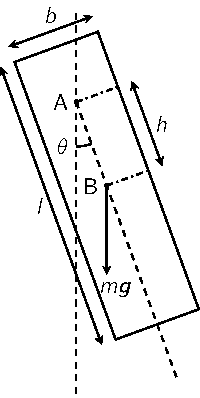
\includegraphics[width=0.15\textwidth]{pendel-oppdatert.pdf}
% Her har vi brukt width=0.15\textwidth for å angi figurbredde som en andel av den delen av arkbredden som inneholder tekst (sidebredde minus marger).
% Hvis du angir bare enten width eller height, beholdes originalfigurens proporsjoner. (Dette anbefales.)
\caption{Her skriver du figurteksten. Merk at denne kommer under figuren. Naturligvis avslutter vi figurteksten med punktum.}
\label{fig:pendel} % Som med ligningen er dette det interne navnet på figuren.
\end{figure}

Husk at figurteksten skal forklare alle de viktige elementene i figuren; leseren skal kunne forstå figuren ved hjelp av figurteksten alene og slippe i lete i brødteksten etter forklaringer. 


\section{Resultater}
Ofte vil vi skrive inn enkeltmålinger i resultatdelen. Da er det viktig å angi usikkerhet. For eksempel kan lengden til pendelen være $l=\SI{1000,015(5)}{\milli\metre}$. 
% Her har vi brukt kommandoen \SI fra siunitx-pakken for å presentere måltall og enheter på en typografisk korrekt måte. Til tall uten enhet trenger vi en kommando med bare ett argument --  da bruker vi \num{<tall>}. Om vi skal oppgi en enhet uten et måltall bruker vi \si{<enhet>}. Søk opp "siunitx" på CTAN for flere detaljer.
% Legg spesielt merke til hvordan man skriver usikkerheten, og hvordan denne kommer frem i den kompilerte pdfen. 
Vi kan også skrive opp usikkerheten separat. I dette tilfellet har vi $\Delta l=\SI{5e-3}{\milli\metre}$. Alternativt kunne vi skrevet denne usikkerheten som $\Delta l=\SI{5e-6}{\metre}$ eller $\Delta l=\SI{5}{\micro\metre}$.

I resultatdelen er det ofte bruk for tabeller for å presentere måledata på en oversiktlig måte. Husk at alle måledata skal oppgis med usikkerhet! Tabell \ref{tab:ckolonner} er et godt eksempel. 
% Merk at vi ikke brukte \autoref i begynnelsen av setningen fordi vi trengte stor forbokstav. 
I \autoref{tab:Skolonner} ser vi et eksempel der den samme tabellen er laget på en litt annen måte. Merk at mens figurtekster står under figurene skal tabelltekster plasseres over tabellene.

% Tabeller i LaTeX kan være litt vanskelig å forstå, men om du studerer eksemplene nøye blir ting forhåpentligvis litt klarere. Det viktigste du må huske på er at tabellene skrives rad for rad. Ampersand angir skiller mellom kolonner, og \\ angir slutten på raden
\begin{table}[tbp]
\centering % Denne kommandoen sentrerer tabellen i kolonnen. 
\caption{Dette er den obligatoriske tabellteksten. Den kommer over tabellen. Husk at de samme reglene gjelder for utforming av tabellteksten som for utforming av figurteksten.}
\label{tab:ckolonner}	% Merkelappen vi vil referere til.
\begin{tabular}{cc} % Her angir det andre argumentet at vi vil ha to senterjusterte kolonner (l = left, c = center, r = right).
\toprule % Horisontal linje som markerer toppen av tabellen
$h$ [\si{\centi\metre}] & $g$ [\si{\metre\per\second\squared}] \\ % Merk at vi skriver variabelnavnene i kursiv. Det er fordi de er matematiske symboler, og har ingenting med at dette er kolonneoverskrifter å gjøre!
\midrule
20  & 9,836\,$\pm$\,0,004 \\ % Kommandoen \, gir et kort mellomrom.
23  & 9,847\,$\pm$\,0,002 \\
29  & 9,839\,$\pm$\,0,008 \\
33  & 9,840\,$\pm$\,0,001 \\
40  & 9,829\,$\pm$\,0,006 \\
\bottomrule
\end{tabular}
\end{table}
% Formatet på denne tabellen er beskrevet i "Retningslinjer for rapportskriving".

% Tabeller med numerisk data skal være linjert på desimalskilletegnet. Ofte kan dette være vanskelig med en enkel c, l eller r. Her kommer heldigvis pakken siunitx til hjelp med det spesielle kolonneformatet S, som vi skal se i denne neste tabellen. 
\begin{table}[tbp]
\centering
\caption{Denne tabellen har identisk innhold som den forrige, men er laget på en litt annen måte.}
\label{tab:Skolonner}
\begin{tabular}{SS[table-format=1.3(1)]} % S = spesielt kolonneformat håndtert av siunitx.
\toprule
{$h$ [\si{\centi\metre}]} & {$g$ [\si{\metre\per\second\squared}]} \\
% Merk deg at kolonneoverskriftene er omsluttet av krøllparanteser i kolonneformatet S!
\midrule
20  & 9,836(4) \\
23  & 9,847(2) \\
29  & 9,839(8) \\
33  & 9,840(1) \\
40  & 9,829(6) \\
\bottomrule
\end{tabular}
\end{table}

Selv om tabeller er hendige, er de ikke alltid den beste løsningen i resultatdelen. Det er for eksempel lettere å se om det er en sammenheng mellom avstanden fra opphengspunktet til massesenteret og verdien og usikkerheten som ble målt for tyngdeakselerasjonen dersom vi plotter resultatene i en figur. Figur \ref{fig:resultater} er et eksempel på dette. Denne presentasjonsformen blir mer aktuell dersom vi har mange resultater. 

\begin{figure}[tbp]
\centering
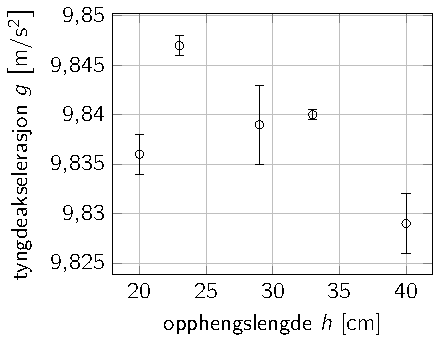
\includegraphics[width=.325\textwidth]{resultater.pdf}
\caption{Denne presentasjonsformen egner seg bedre til å tydeliggjøre trender i datagrunnlaget. Her kan det se ut som om verdien vi måler for $g$ og usikkerheten i målingene er relativt uavhengig av $h$.}
\label{fig:resultater}
\end{figure}

% Figurene og tabellene vi har brukt så langt har vært avgrenset til én kolonnebredde. Om vi trenger tabeller eller figurer som dekker hele sidebredden får vi det ved å bruke miljøene figure* og table*. 

\section{Diskusjon}
Rapportskriving i \LaTeX\ gir mange muligheter. Selv om det er endel tekniske finesser som skal på plass er det viktig å huske på at god skriving og godt språk ligger til grunn for å skrive en god rapport. 

\section{Konklusjon}
Nå har vi gitt endel eksempler på formatering. For å mestre \LaTeX\ er det bare én ting som gjelder -- trening. Last ned kildefilene og lek med de ulike elementene. Sitter du fast er det som regel noen som har hatt de samme problemene før deg. Det meste av dokumentasjon er å finne på \href{http://www.ctan.org/}{CTAN}. Spørsmål og svar er å finne på \href{http://tex.stackexchange.com/}{\LaTeX\ StackExchange}. Lykke til!

% Her kommer referanselisten
\begingroup
\begin{center}
\rule{2cm}{.4pt} % Vi markerer starten på referanselisten med en horisontal strek
\end{center}
\makeatletter
\@beginparpenalty=10000 % Vi setter en høy straff for kompilatoren om den setter inn et sideskift mellom streken og starten på referanselisten.
\makeatother
\bibliographystyle{babunsrt}
\bibliography{referanseliste}
\endgroup

\end{document}